\documentclass[11pt]{preprint}

\setlength{\topmargin}{0mm} \setlength{\oddsidemargin}{0mm}
\setlength{\textwidth}{160mm} \setlength{\textheight}{215mm}

\usepackage{amssymb,amsmath,amscd,amsthm}
\usepackage{graphics}
\usepackage{tikz}

\def\enumb{\begin{enumerate}}
\def\enume{\end{enumerate}}
\def\itemb{\begin{itemize}}
\def\iteme{\end{itemize}}
\def\integers{\mathbb{Z}}

\def\multiset#1#2{\ensuremath{\left(\kern-.3em\left(\genfrac{}{}{0pt}{}{#1}{#2}\right)\kern-.3em\right)}}



\newtheorem{proposition}{Proposition}
\newtheorem{theorem}{Theorem}

\title{Discrete Mathematics, 2016 Fall - Worksheet 24}
\author{Instructor: Zsolt Pajor-Gyulai, CIMS}



\begin{document}

\maketitle

In all of the above problems explain your answer in full English sentences.

\enumb
\item For which values of $n$ is the complete graph $K_n$ Eulerian?
\item Let $G$ be a connected graph that is not Eulerian. Prove that it is possible to add a single vertex to $G$, together with some edges from this new vertex to some old vertices such that the new graph is Eulerian.

\item Let $G$ be the graph in the following figure.
\begin{figure}[ht]
\centering
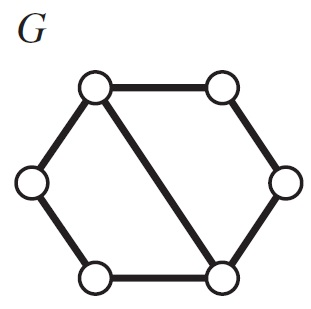
\includegraphics[scale=0.5]{Color1.jpg}
\end{figure}
Please find $\chi(G)$.
\item Let $G$ be a graph and let $v$ be a vertex of $G$. Prove that
\[
\chi(G-v)\leq \chi(G)\leq \chi(G-v)+1
\]
\item Let $G=K_{n,m}$. Determine $|V(G)|$ and $|E(G)|$.
\item Let $G$ be a graph with $n$ vertices. Prove that $\chi(G)\chi(\bar{G})\geq n$.
\enume
\end{document}